\documentclass{csc_assignment5}
\usepackage[utf8]{inputenc}
\usepackage[letterpaper, portrait, margin=1in]{geometry}
\usepackage{calc}  % arithmetic in length parameters
\usepackage{enumitem}  % more control over list formatting
\usepackage{fancyhdr}  % simpler headers and footers
\usepackage{lastpage}  % for last page number
\usepackage{relsize}  % easier font size changes
\usepackage[normalem]{ulem}  % smarter underlining
\usepackage{url}  % verb-like typesetting of URLs
\usepackage{xfrac}  % nicer looking simple fractions for text and math
\usepackage{amsmath}
\usepackage{amssymb}
\usepackage{tikz}
\usepackage{algorithm}
\usepackage{algorithmic}
\usepackage{graphicx}
\usepackage{listings}
\graphicspath{{/}}
\usepackage[export]{adjustbox}
\usepackage{enumitem}
\usepackage{subcaption}
\usepackage{esvect}
\lstset{breaklines=true}

% ----------------------------------------------------------------
% TODO: Enter the assignment number, your name, and your student number below
% ----------------------------------------------------------------
\AssignmentName{Final Project Report}
\StudentName{Akhil Gupta and Satbir Mangat}
\StudentNumber{1000357071 and 1000547330}

% ----------------------------------------------------------------
\begin{document}
\begin{description}

\item[NOTE:]
All the work in this project was done together so we will be submitting only one report.
\item[Problem Statement:]
For our final project, we chose to work on Project 3. Our task was to do pixel-level labelling with a set of semantic classes. In particular, we are to:
\begin{enumerate}
\item Automatically label each pixel as either ``person'' or ``background''
\item Automatically label each pixel as either: ``background'', ``skin'', ``hair'', ``t-shirt'', ``shoes'', ``pants'', ``dress''.
\end{enumerate}

\item[SOLUTION:]
This is how we chose to tackle the problem:
\begin{enumerate}
\item We create superpixels for each image
\item Compute feature vectors and labels for the training data and also get features per image to map the superpixel segments to the correct iamge
\begin{enumerate}
\item We used the first 784 pixels from each superpixels segment to form a 28 x 28 square
\item Compute HOG features on each square
\item Used the HOG features as the features for our NN to perform classification on all segments
\item We use a variable $numberOfClasses$ which can be set to 7 (background, skin, hair, etc.) or 2 (person, background)
\item Then label all pixels in each image
\end{enumerate}
\item We repeat Step 2 for validation data as well as test data
\item Train a MLP Classifier using training data with 3 hidden layers of 200 neurons in each layer and max\_iter=10,000
\item We predict the output of our Neural Network on train, test and validation images and save the predictions in folder $results-seg$
\item Output of our NN is attached after CODE (complete output is attached on MarkUs as $results-seg.zip$. (We are submitting the first 180 images because our code only runs on 180 images)
\end{enumerate}

\item[CHALLENGES:] 
Below is a list of some challenges we faced:
\begin{enumerate} 
\item Lack of computational resources
\item Not enough time to fine-tune hyperparameters
\item Only used 784 pixels of each superpixel segment 
\item We know our code works better on person vs background; trying to improve on the other case
\end{enumerate}

\item[HOW TO RUN:]
Place $code.py$ in the project3 folder along with images and labels. run 'python code.py' \\\\

\item[CODE:] Code snippet attached below (also on MarkUs as code.py): 
\begin{lstlisting}[language=Python]
import numpy as np
from skimage.segmentation import slic
from sklearn.neural_network import MLPClassifier
from skimage.feature import hog
import cv2
import glob

# Label all pixels and generate segmentation images.
def main():
    # Multiclass (i.e clothes).
    segmentation(False)
    # Binary (i.e person).
    segmentation(True)

def segmentation(personOnly = False):
    # Open all images.
    images = [cv2.imread(f) for f in glob.glob("images/*.jpg")]
    trainImgs = images[:300]
    valImgs = images[300:360]
    testImgs = images[360:]
    
    labelType = 'clothes'
    labelFactor = 14
    if personOnly:
        labelType = 'person'
        labelFactor = 255
        
    # Open all label images.
    labelImages = [cv2.imread(f, cv2.IMREAD_GRAYSCALE) / labelFactor
                   for f in glob.glob('labels/*_' + labelType + '.png')]
    trainLabels = labelImages[:300]
    valLabels = labelImages[300:360]
    testLabels = labelImages[360:]
    
    # Compute superpixels for each image.
    superpixels = [slic(img.astype(float)) for img in images]
    trainSP = superpixels[:300]
    valSP = superpixels[300:360]
    testSP = superpixels[360:]
    
    # Compute feature vectors and labels for training data. Also get the
    # Features per image to map the segments to the correct image.
    
    trainFeatures, trainLabels, trainFPI = computeAllFeaturesAndLabels(trainImgs, trainLabels, trainSP, personOnly)
    
    # Compute feature vectors and labels for validation data. Also get the
    # Features per image to map the segments to the correct image.
    valFeatures, valLabels, valFPI = computeAllFeaturesAndLabels(valImgs, valLabels, valSP, personOnly)
    
    # Compute feature vectors and labels for test data. Also get the
    # Features per image to map the segments to the correct image.
    testFeatures, testLabels, testFPI = computeAllFeaturesAndLabels(testImgs, testLabels, testSP, personOnly)
    
    # Train clasifier.
    clf = MLPClassifier(hidden_layer_sizes=(200, 200, 200), max_iter=10000)
    clf.fit(trainFeatures, trainLabels)
    
    # Predict validation images.
    predictionsVal = clf.predict(valFeatures)
    predictedImgsVal = labelPixels(predictionsVal, valSP, valFPI)
    
    # Predict Test images.
    predictionsTest = clf.predict(testFeatures)
    predictedImgsTest = labelPixels(predictionsTest, valSP, valFPI)
    
    # Predict train images.
    predictionsTrain = clf.predict(trainFeatures)
    predictedImgsTrain = labelPixels(predictionsTrain, valSP, valFPI)
    
    # Save all the predicted images.
    saveSegImages(predictedImgsTrain + predictedImgsVal + predictedImgsTest,
                  personOnly, labelFactor, 1)
    
    
# Compute the feature vectors and labels for all 'images' using 'labelImages' and 'superpixels'.
def computeAllFeaturesAndLabels(images, labelImages, superpixels, personOnly):
    # Keep track of the number of features per image.
    featuresPerImage = []
    # List of all feature vectors of all images.
    allFeatures = []
    # List of all labels of all images.
    allLabels = []
    
    for i in range(len(images)):
        curFeatures, labels = computeFeaturesAndLabelsPerImage(images[i], labelImages[i], superpixels[i], personOnly)
        featuresPerImage.append(len(curFeatures))
        allFeatures += curFeatures
        allLabels += labels
    
    return allFeatures, allLabels, featuresPerImage

# Compute the feature vectors and labels for 'image' using 'labelImage' and 'superpixels'.
def computeFeaturesAndLabelsPerImage(image, labelImage, superpixels, personOnly):
    # Use this many pixels squared of each segment.
    SEG_SIZE = 28
    features= []
    labels = []
    
    # Convert image to grayscale.
    image = cv2.cvtColor(image, cv2.COLOR_BGR2GRAY)
    
    # Loop through each segment label in 'superpixels'.
    for segLabel in range(np.max(superpixels) + 1):
        # Get the first 'SEG_SIZE' squared pixel coordinates in the current segment (y, x).
        segCoords = np.argwhere(superpixels == segLabel)[:SEG_SIZE ** 2]
        Xs = segCoords[:, 1]
        Ys = segCoords[:, 0]

        # Reshape the segment into a square.
        segment = image[Ys, Xs].reshape(SEG_SIZE, SEG_SIZE)
        featureVector = hog(segment)
        features.append(featureVector)
        
        # Most common label in this segment.
        labelPixelVal = np.argmax(np.bincount(labelImage[Ys, Xs]))
        # One-hot encoded value.
        numberOfClasses = 7
        if personOnly:
            numberOfClasses = 2
        label = np.zeros(numberOfClasses)
        # Changing the pixel value of the label to be in range 0-6 (or 0-1).
        label[min(labelPixelVal, 6)] = 1
        labels.append(label)
        
    return features, labels

# Label all pixels in all images.      
def labelPixels(labels, superpixels, featuresPerImage):
    # Contains all the labeled images.
    labeledImages = []
    # Starting index of the labels for the current image.
    start = 0
    for i in range(len(featuresPerImage)):
        # Ending index of the labels for the current image.
        end = start + featuresPerImage[i]
        labeledImages.append(labelPixelsSingleImage(labels[start: end], superpixels[i]))
        start = end
    
    return labeledImages

# Label individual pixels based on what segment they belong to indicated by 'superpixels'. 
def labelPixelsSingleImage(labels, superpixels):
    nonZeros = 0
    labeled = np.copy(superpixels)
    # The index of labels corresponds to the segment label in its image.
    for i in range(len(labels)):
        # Assign the label to all pixels in the segment.
        labeled[labeled == i] = np.argmax(labels[i])
        if np.argmax(labels[i]) > 0:
            nonZeros += 1
     
    return labeled

# Save the segmented images.
def saveSegImages(images, personOnly, labelFactor, firstImgNum):
    segType = 'clothes'
    if personOnly:
        segType = 'person'
    
    for i in range(len(images)):
        fileName = 'results-seg/' + format(i + firstImgNum, '04') + '_' + segType + '.png'
        cv2.imwrite(fileName, images[i] * labelFactor)

if __name__== "__main__":
    main() 
    
*** OUTPUT ATTACHED BELOW ***
\end{lstlisting}

\newpage
\item[OUTPUT FROM OUR NN:]
We have attached a few images below:
\begin{figure}[h!]
    \centering
    \begin{subfigure}[b]{0.3\textwidth}
        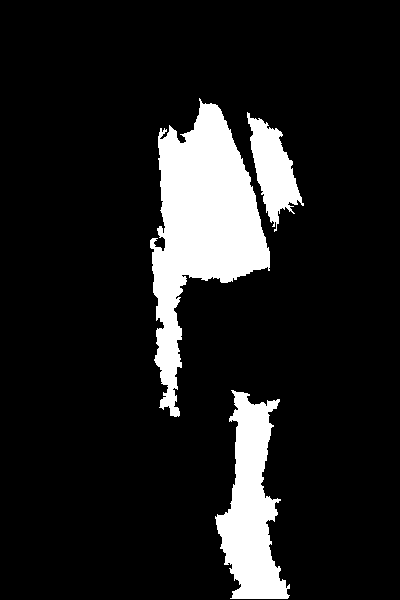
\includegraphics[width=\textwidth]{results-seg/0067_person.png}
        \caption{0067 person output}
    \end{subfigure}
    \quad
    \begin{subfigure}[b]{0.3\textwidth}
        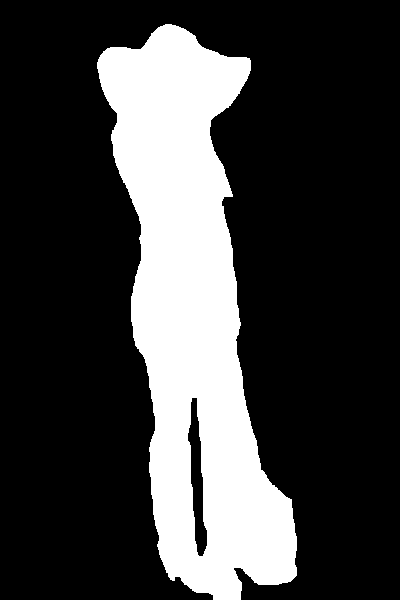
\includegraphics[width=\textwidth]{labels/0067_person.png}
        \caption{0067 person ground truth}
    \end{subfigure}
\end{figure}

\begin{figure}[h!]
    \centering
    \begin{subfigure}[b]{0.3\textwidth}
        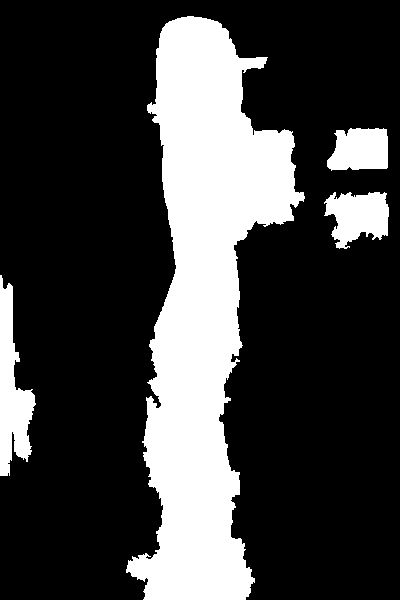
\includegraphics[width=\textwidth]{results-seg/0071_person.png}
        \caption{0071 person output}
    \end{subfigure}
    \quad
    \begin{subfigure}[b]{0.3\textwidth}
        
\includegraphics[width=\textwidth]{labels/0071_person.png}
        \caption{0071 person ground truth}
    \end{subfigure}
\end{figure}

\begin{figure}[h!]
    \centering
    \begin{subfigure}[b]{0.3\textwidth}
        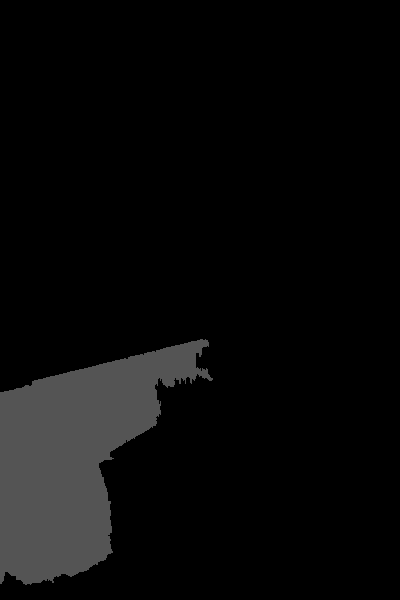
\includegraphics[width=\textwidth]{results-seg/0134_clothes.png}
        \caption{0134 clothes output}
    \end{subfigure}
    \quad
    \begin{subfigure}[b]{0.3\textwidth}
        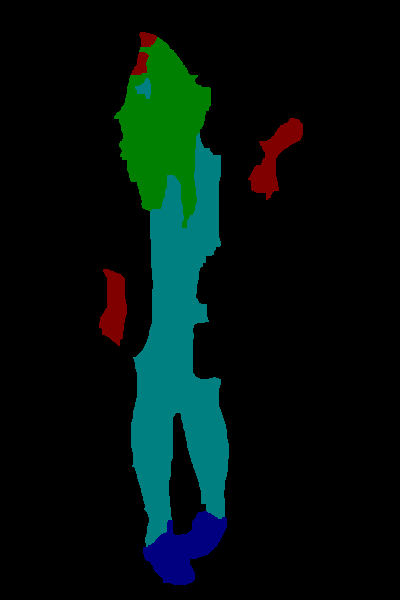
\includegraphics[width=\textwidth]{labels/0134_clothes.png}
        \caption{0134 clothes ground truth}
    \end{subfigure}
\end{figure}

\begin{figure}[h!]
    \centering
    \begin{subfigure}[b]{0.3\textwidth}
        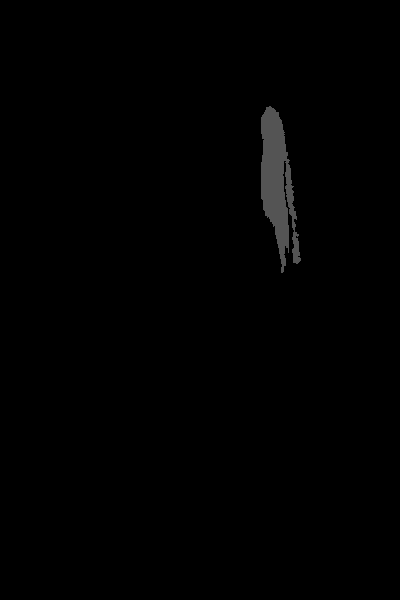
\includegraphics[width=\textwidth]{results-seg/0146_clothes.png}
        \caption{0146 clothes output}
    \end{subfigure}
    \quad
    \begin{subfigure}[b]{0.3\textwidth}
        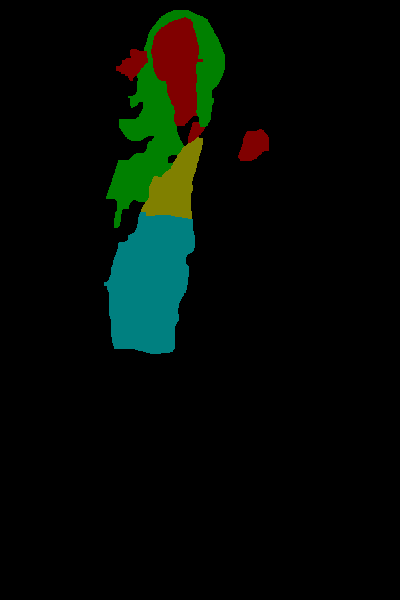
\includegraphics[width=\textwidth]{labels/0146_clothes.png}
        \caption{0146 clothes ground truth}
    \end{subfigure}
\end{figure}



\end{description}
\end{document}
  
  



